\newpage
\begin{center}
	\textbf{\large 1. ВВЕДЕНИЕ В ПОРТФЕЛЬНУЮ ТЕОРИЮ}
\end{center}
\refstepcounter{chapter}
\addcontentsline{toc}{chapter}{1. ВВЕДЕНИЕ В РЫНОК КРИПТОВАЛЮТ}

\section{Основные понятия}

Портфельный анализ берет свое начало с выхода статьи Гарри Марковица в 1952 г \cite{markowitz}. Подход Марковица начинается с предположения что инвестор в 
настоящий момент времени имеет конкретную сумму денег для инвестирования. Эти деньги будут инвестированы на определенный промежуток
времени, который назывется \textbf{периодом инвестирования}. В конце периода инвестор продает активы купленные в
ранее. 
Набор приобретенных активов иначе называют \textbf{инвестиционным портфелем}. Поэтому проблема выбора и распределения
средств по активам имеет название \textbf{проблемой выбора инвестиционного портфеля}.

Пусть цены актива на начало и конец периода инвестирования равны $S^0$ и $S^1$ соотвественно.
Определим \textbf{доходность актива} (Return) $r$ за период инвестирования как
\[
	r = \frac{S^1 - S^0}{S^0}
\]

При формировании портфеля в начальный момент времени, инвестор должен иметь в виду что доходность активов
за будущий период владения заранее неизвестна. То есть он вынужден принимает решение о выборе портфеля исходя из 
своих ожидаемых доходностей активов. 

Если инвестор ставит задачей максимизировать доходность портфеля, то в этом случае его портфель должен состоять из единственного
актива с наибольшей ожидаемой доходностью. Марковиц отмечает, что такой подход является неразумны, потому что типычный инвестор
хоть и желает чтобы <<доходность была высокой>>, но одновременно требует чтобы <<доходность была настолько определенной насколько
это возможно>>. Это означает, что инвестор, стремясь одновременно максимизировать доходность и минимизировать риск 
(неопределенность), имеет две противоречащие друг другу цели. Подход Марковиа к принятию решения дает возможность адекватно 
учесть обе эти цели.

Имея $N$ доступных активов можно сформировать бесконечно много портфелей. Это множество называют \textbf{достижимым}. 
Как инвестору в этих условиях выбрать портфель? Логичными являются следующие принципы при формировании портфеля:
\begin{itemize}
	\item Из двух портфелей с одинаковым риском, инвестор выберет порфтель с большей ожидаемой доходностью
	\item Из двух портфелей с одинаковой доходностью, инвестор выберет портфель с меньшим риском
\end{itemize}
Другими словами, из достижимого множества портфелей инвестор склонен выбирать парето-оптимальные портфели.
Множество оптимальных портфелей иначе называют \textbf{эффективным множеством}. Достижимые портфели не из 
эффективного множества называют \textbf{неэффективными портфелями}.

Вопрос выбора конкретного портфеля из эффективного множества остается на стороне инвестора. Здесь он уже руководствуется
своей внутренней толерантностю к риску. Обычно достаточно зафиксировать приемлимый уровень риска внутри достижимого множества
и выбрать портфель с соответсвующей доходностью. 


\begin{figure}[H]
	\centering
	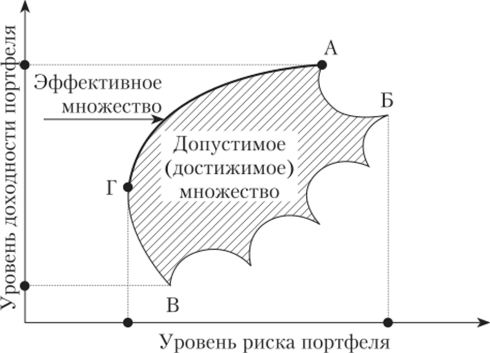
\includegraphics[width=\textwidth]{port_set.png}
	\caption{Множество портфелей}
	\label{fig:port_set}
\end{figure}


